Studying the Inertial electrostatic confinement fusor at DTU. Measurements of neutron counts and the spectral line width are made as a function of the voltage and current. To this, the emission spectrum of the gas are also measured.
\subsection{Plasma light emission and spectral line}
When doing spectroscopy on a plasma of an unknown gas. Optical dispersion splits up the spectrum of light into lines which are then recorded using a detector. This detector measures the frequency/wavelength of the light and the intensity of the light. Thus a plot with the wavelength along the x-axis vs the intensity along the y-axis are produced. Meanwhile peaks are present on the recording where each peak are subject to broadening effects. Considering the Doppler effect, each photon's frequency will be shifted since the particles(which are the emitters) are moving at fast speeds(the Doppler shift increases with speed). Therefore if each particle where moving in the same direction the entire intensity peak would be shifted. But since the particles are moving more or less isotropically, the peaks are not shifted but rather broadened around the normal emission wavelength. To this it is also noted that the Doppler broadening increases if particles are moving faster.\\
Considering \cref{fig:Spectro}, a spectral line is shown with a central wavelength of around $\SI{656}{\nano\meter}$ which correspond to the accepted value of hydrogen light emission\footnote{https://en.wikipedia.org/wiki/Hydrogen_spectral_series}. Meanwhile the spectral lines of Deuterium only differs by a factor of $1.000272$\footnote{https://en.wikipedia.org/wiki/Deuterium#Spectroscopy}.
\begin{figure}
	\centering
	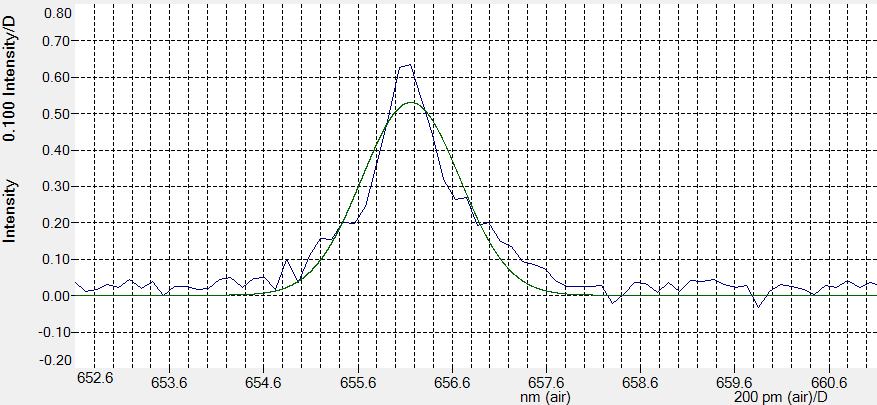
\includegraphics{Figures/D_linje.png}
	\caption{Spectral line for deuterium measured in the fusor.}
	\label{fig:Spectro}
\end{figure}